\documentclass[12pt]{article}
\usepackage[spanish]{babel}
\usepackage[utf8x]{inputenc}
\usepackage{tabularx} % extra features for tabular environment
\usepackage{amsmath}  % improve math presentation
\usepackage{graphicx} % takes care of graphic including machinery
\usepackage{geometry} % decreases margins
\usepackage{cite} % takes care of citations
\usepackage[final]{hyperref} % adds hyper links inside the generated pdf file
\usepackage{booktabs}
\usepackage{subcaption}
\usepackage{fancyhdr}
\usepackage{parskip}
\usepackage{amssymb, amsmath} % Paquetes matemáticos de la American Mathematical Society
\usepackage{float}
%\usepackage{showframe}

\hypersetup{
	colorlinks=true,       % false: boxed links; true: colored links
	linkcolor=black,        % color of internal links
	citecolor=black,        % color of links to bibliography
	filecolor=magenta,     % color of file links
	urlcolor=blue         
}
\spanishdecimal{.}

%++++++++++++++++++++++++++++++++++++++++
%Content

\title{\textbf{Ejemplo Señal Periódica Diente de Sierra con Espacios Variable}}

\begin{document}
    \maketitle
    \section*{Ejemplo}
        Encontrar la serie de Fourier de la forma de onda triangular que se muestra  
        en la figura. La ecuación para esta forma de onda es:
        \begin{equation*}
            x(t)=\begin{cases}
                t & 0 < t \leq 0,5 \\
                0 & 0,5 < t \leq 1.0                
            \end{cases}
        \end{equation*}
        \begin{figure*}{H}
            \centering
            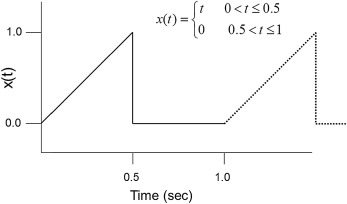
\includegraphics{img/figure1.jpg}
            \caption{Una forma de onda de medio triangulo usado en el ejemplo.}
        \end{figure*}
        Encuentre los primeros cuatro componentees de magnitud y fase (es decir, m=1,2,3,4).
        Construya gráficas de frecuencia de los componentes de magnitud.\\
    \section*{Solución}
        Use las ecuaciónes 1 y 2 para encontrar los coeficientes $a_{n}$ y $b_{m}$. Luego 
        convierta a magnitud, $M_{n}$ y fase, $\theta_{n}$, usando las ecuaciones 3 y 5. 
        Gradique $M_{n}$ y $\theta_{n}$ contra la frecuencia asociada, $f=nf_{0}$.\\
        \\
        Empiece por evaluar los coeficientes de seno o coseno; comenzamos con los 
        coeficientes de seno usando la Ecuación 2:
        \begin{equation*}
            b_{n}=\frac{2}{T} \int_{T} x(t)sin(2\pi nf_{0}t)dt
        \end{equation*}
\end{document}